This chapter is devoted to the evaluation of Particle Q Learning on classic benchmark problems, both in the tabular and in the function approximation cases. In Section ~\ref{sec:tabular_experiments} we show the results of experiments in the tabular case for classic problems found in the literature. Section ~\ref{sec:atari_experiments} describes the experiments performed in the \emph{Arcade Learning Environment} (ALE) ~\cite{Bellemare:2013:ALE:2566972.2566979}, a classic benchmark in the Deep RL literature. 
\section{Tabular Case} \label{sec:tabular_experiments}
This section is devoted to experiments conducted in finite domains where the tabular version of the algorithm can be used. The experiments are done in 6 different domains taken from the literature on efficient and deep exploration. Combining  the two policies (VPI policy and Weighted Policy) with the two update methods (Maximum Mean Updating and Weighted Updating) proposed in the previous chapter we propose four versions of Particle Q-learning. We compare the results produced using these algorithms with the ones produced from different variations of two algorithms from the literature:
\begin{itemize}
\item Q-learning with $\epsilon$-greedy or Boltzmann exploration,
\item Bootstrapped Q-learning with the Bootstrapped policy defined in ~\cite{DBLP:journals/corr/OsbandBPR16} and with the Weighted policy discussed in the previous chapter.
\end{itemize}
For all algorithms we have also considered their ``double'' versions, \ie modifications of the algorithms that use two Q-tables as in ~\cite{Hasselt:2016:DRL:3016100.3016191}. The results of using the ``double'' versions are shown in Appendix~\ref{app:appendixA} 
\subsection{Evaluation Metrics}
In this thesis, we addressed the exploration vs. exploitation dilemma by maintaining Q-distributions and using them to perform more informed decisions. A reinforcement learning agent needs exploration to learn an optimal policy faster in complex domains, but also not to get stuck in sub-optimal policies in domains that except them, and where discovering the optimal policy might be ``trickier''. For this purpose we test our algorithms in 6 domains, some of them designed to be ``tricky'', and some classical navigation problems. We compare algorithms by looking at the learning curve, \ie mean scores collected as a function of the training time. Algorithms that explore better, should not only show faster increasing curves, but also not get stuck in sub-optimal solutions. We show the mean scores over multiple runs, by shadowing around the curves to show also 95\% confidence interval.\par
We will also discuss how the Q-distributions maintained by the agent progress during learning. As we mentioned in the previous Chapter, as learning continues, the distributions should shrink to the true Q-value. We note that if the distributions shrink too quick, the agent might be stuck in a suboptimal policy. For this purpose we will show the following:
\begin{itemize}
\item Particle positions as learning progresses, to see if they do in fact converge,
\item Variance of the Q-distributions, which should converge to 0,
\item Probability of exploration, \ie probability of choosing an action different than the greedy one.
\end{itemize}
The first two of these curves are defined for each $(s,a)$ pair, whereas the last curve is defined for each state.
\subsection{Experimental Setup}
We train each agent for 100 episodes, the length of each episode is domain dependent. During the training periods we collect the rewards and use them to calculate the \emph{online scores}. After each training period, we ``turn off'' exploration and evaluate the policies learned by the agent. The length of the evaluation episodes is the same as the training episodes. We use the rewards collected during evaluation to calculate the \emph{offline scores}. We perform this process in each domain, for each algorithm considered and show the mean scores of 10 runs. We calculate the undiscounted scores, even though we use a discount factor in each domain during learning.\par
For our particle algorithms, we initialize the particles equally spaced in an interval $[q_{min}, q_{max}]$, for each state action-pair. The range of this interval is problem dependent and we see these hyper parameters as a way to incorporate prior knowledge about the domain. We consider Bootstrapped Q-learning with two policy models, the Bootstrapped policy defined in \cite{DBLP:journals/corr/OsbandBPR16} and the weighted policy. We initialize the Q-tables with values drawn from a Gaussian distribution with parameters $\mu=\frac{q_{min}+q_{max}}{2},\sigma=q_{max}-q_{min}$. Furthermore, we consider Q-learning algorithm with $\epsilon$-greedy and Boltzmann exploration. In both Q-learning versions, the Q-table is initialized to 0.\par
For all algorithms we use a \emph{exponentially decaying} learning rate given by:
\begin{equation}
\label{eq:exponential_decay}
\alpha(s,a) = \frac{b}{t(s,a)^a},
\end{equation}
where $t(s,a)$ is the visit count for state-action pair $(s,a)$, $b$ is the initial value which we set to 1 and $a$ is the \emph{decay exponent}. For all our experiments we used $a=0.2$, as it gave us better results.\par
For the Q-learning algorithms we had to chose also the schedules for $\epsilon$ and $\beta$, for $\epsilon$-greedy and Boltzmann exploration respectively. For $\epsilon$ we used an exponetially decaying schedule as in (\ref{eq:exponential_decay}) with $b=1$ and $a=0.5$ whereas for the Boltzmann policy we used an exponentially decaying $\beta$ with initial value, $b=1.5q_{max}$ and decay exponent, $a=0.5$. 
\subsection{Chain Domain}
The first domain we describe, taken from~\cite{Dearden98bayesianq-learning}, is shown in Figure~\ref{fig:chain_domain}. The domain is composed of 5 states, labeled from 1 to 5. The agent can choose between two actions in each domain, labeled as $a$, $b$ (represented in the figure as the edges). The labels in the edges represent the action executed and the reward collected from the transition. With probability $p=0.2$ each action ``fails'' and the opposite action is executed instead, \ie we observe reward $r$ and next-state $s'$ of the opposite action. The domain is designed to test exploration approaches. Assuming a discount factor $\gamma=0.99$, the optimal policy is to always execute action $a$ to receive the high reward at the last state. If the agent does not explore enough it could be stuck in the suboptimal policy of executing always $b$ and collecting the smaller reward of 2.
\begin{figure}
 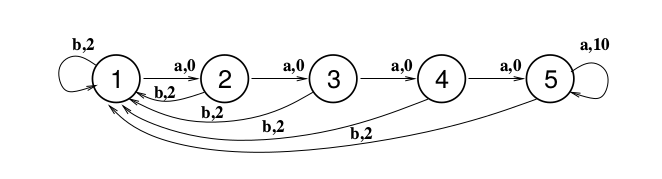
\includegraphics[width=\linewidth]{chain_domain.png}
 \caption{Chain domain taken from ~\cite{Dearden98bayesianq-learning}.}
 \label{fig:chain_domain}
\end{figure}
\begin{figure}
 \includegraphics[width=\linewidth]{Chain/learning_curve.pdf}
 \caption{Online (left) and offline (right) scores in the Chain domain.}
 \label{fig:chain_learning_curve}
\end{figure}
Figure~\ref{fig:chain_learning_curve} shows the results of our tests in the Chain domain. We trained each agent for 100 episodes of 1000 timesteps, for a total of 100000 timesteps. The scores collected during training are shown in the left plots. After each training periods, we evaluated the agents for another 1000 steps. During evaluation agents stopped exploring and followed the greedy policies instead. This was done to evaluate the policies derived if training finished at that moment. The plots show the mean score of 10 independent runs and the shaded regions around the line, represent the 95\% confidence interval of the mean.\par
\begin{figure}
\centering
\begin{subfigure}{\linewidth}
  \centering
  \includegraphics[width=\linewidth]{Chain/particles_weighted-weighted.pdf}
  \caption{}
  \label{fig:chain_particles_weighted_weighted}
\end{subfigure}%

\bigskip
\centering
\begin{subfigure}{\linewidth}
  \centering
  \includegraphics[width=\linewidth]{Chain/particles_vpi-mean.pdf}
   \caption{}
   \label{fig:chain_particles_vpi_mean}
\end{subfigure}
\caption{Evolution of the particles in the first state of the Chain domain during the learning process for the Particle Q-learning algorithm with weighted policy and weighted update (a), and VPI policy and maximum mean update (b). The optimal action \emph{a} is shown on the left, while the suboptimal action \emph{b} is shown on the right on both (a) and (b).}
\label{fig:chain_particle_evolution}
\end{figure}
We can understand immediately from the picture that simple exploration strategies, like Boltzmann, fail to solve this simple domain. If we consider the online case, \ie how the agent behaves during training, our algorithm, Particle Q-learning, used with VPI policy and maximum mean update, has the best performance, scoring the maximum possible since the beginning of learning. We can note that bootstrapped Q-learning (BQL) starts good at the beginning and then its performance is surpassed by the performance of our algorithms using the weighted policy, with both update methods (weighted and maximum mean). We evaluated also another version of BQL, which used the weighted policy. We can see that in the online case, this algorithm did not perform well. It is interesting that, in the offline evaluation, BQL performed really well since the beginning. This means that while it learned the optimal policy quickly, it failed to send exploration to zero fast enough. This is something we will see also in the next experiments.\par
We will now discuss how the particles evolve during time. As mentioned before the desired behaviour is that the particles converge to the real Q-value. Obviously, at this point, the algorithm will stop exploring. Figure~\ref{fig:chain_particle_evolution} shows the evolution of the particles in the first state during learning for two versions of our algorithm. We could show these plots for all state-action pairs but for space considerations we are only showing the particles in the first state for both actions. We made this choice because the first state is the most difficult state to learn because it is the closest to the small reward and the furthest from the high reward. \par
\begin{figure}
\centering
\begin{subfigure}{\linewidth}
  \centering
  \includegraphics[width=\linewidth]{Chain/std_weighted-weighted.pdf}
  \label{fig:chain_std_weighted_weighted}
  \caption{}
\end{subfigure}

\bigskip
\centering
\begin{subfigure}{\linewidth}
  \centering
  \includegraphics[width=\linewidth]{Chain/std_vpi-mean.pdf}
  \label{fig:chain_std_vpi_mean}
  \caption{}
\end{subfigure}
\caption{Standard deviation of the particles as a function of the learning timestep for the Particle Q-learning algorithm with weighted policy and weighted update (a), and VPI policy and maximum mean update (b). Once again, the optimal action \emph{a} is shown on the left, while the suboptimal action \emph{b} is shown on the right on both (a) and (b).}
\label{fig:chain_std_evolution}
\end{figure}
In Figure~\ref{fig:chain_particles_weighted_weighted}, we can see that for Particle Q-learning with weighted policy and weighted update (PQL\_W\_W), the particles shrink during learning, and after the step 20000, action $b$ is not explored anymore and its particles remain constant. Particle Q-learning with VPI policy and maximum mean update (PQL\_V\_M), shown in Figure~\ref{fig:chain_particles_vpi_mean}, shrinks the particles much faster in the optimal action (left subplot) whereas never shrinks the ones of the suboptimal action. This means that VPI policy stops exploring actions before the uncertainty of their Q-value goes to zero. In this simple domain this gave higher results faster, but in more complicated domains this might lead to premature convergence of the algorithm. This can be seen also in Figure~\ref{fig:chain_std_evolution} where the standard deviation of the particles in the same state is shown for both algorithms. While in the PQL\_W\_W case the standard deviation goes to zero for both actions, in the PQL\_V\_M case only the first action goes to 0. The particles of action $b$ remain spread and the standard deviation remains constant. This is explained by the fact that VPI policy does not consider this action worth exploring even though it is not completely sure about its value, as explained in the previous chapter. we note that while PQL\_V\_M brought good results in this domain, the fact that the actions are not fully explored, and as a result the particles do not shrink, might bring premature convergence in more complex domains.\par
\begin{figure}
  \centering \includegraphics[width=\linewidth]{Chain/prob_weighted-weighted.pdf}
\caption{Probability of exploration as a function of the learning timestep for the Particle Q-learning algorithm with weighted policy and weighted update in the Chain domain.}
\label{fig:chain_prob_evolution}
\end{figure}
Finally we show how the probability of exploration evolves as learning continues. Again we recall that the probability should go to 0, as we go closer the true Q-value. Figure~\ref{fig:chain_prob_evolution} displays our results for PQL\_W\_W. Again we consider just the first state. Same plots could be shown for all states of the domain. We can see that  the probability of exploration goes to 0.

\subsection{Loop Domain}
The second domain we consider, shown in Figure ~\ref{fig:loop_domain}, is also taken from~\cite{Dearden98bayesianq-learning}. Similar to the first domain, the agent has 2 available actions in each of the 9 states. The name comes from the fact that, starting from the initial state 0, the agent has to choose between the two loops available. All rewards are 0, except the last transitions of the loops. The agent has to learn to perform the left loop, which gives the highest reward, but the right loop, although suboptimal, is easier to reach. An agent that does not explore enough might be stuck in the suboptimal loop.\par
\begin{figure}
 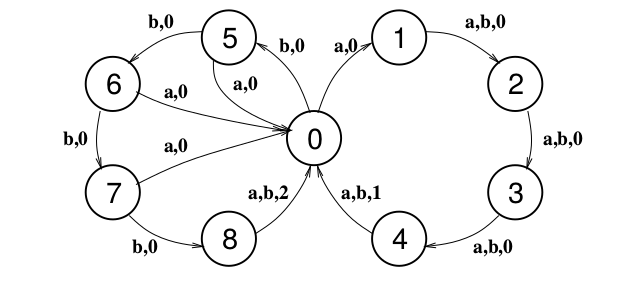
\includegraphics[width=\linewidth]{loop_domain.png}
 \caption{Loop domain taken from ~\cite{Dearden98bayesianq-learning}.} 
 \label{fig:loop_domain}
\end{figure}
\begin{figure}
 \includegraphics[width=\linewidth]{Loop/learning_curve.pdf}
 \caption{Online and offline scores in the Loop domain.}
 \label{fig:loop_learning_curve}
\end{figure}
Figure~\ref{fig:loop_learning_curve} shows the results of our tests in the Loop domain. Again we trained each agent for 100 episodes of 1000 timesteps, for a total of 100000 timesteps and display the online and offline undiscounted scores. This domain is slightly more simple than Chain. Indeed simple exploration approaches like Boltzmann or $\epsilon$-greedy perform well in this domain. Nonetheless, PQL with VPI policy performs best in both offline and online cases, while the versions using weighted policy learn slower due to the fact that they explore actions until they are sure about their value. We can see that boostrapped Q-learning starts better than these algorithms, but its performance is surpassed later. We will also discuss the behaviour of the particles as before. \par
\begin{figure}
\centering
\begin{subfigure}{\linewidth}
  \centering
  \includegraphics[width=\linewidth]{Loop/particles_weighted-weighted.pdf}
  \label{fig:loop_particles_weighted_weighted}
  \caption{}
\end{subfigure}%

\bigskip
\centering
\begin{subfigure}{\linewidth}
  \centering
  \includegraphics[width=\linewidth]{Loop/particles_vpi-mean.pdf}
  \caption{}
  \label{fig:loop_particles_vpi_mean}
\end{subfigure}
\caption{Evolution of the particles in the first state of the Loop domain during the learning process for the Particle Q-learning algorithm with weighted policy and weighted update (a), and VPI policy and maximum mean update (b). The optimal action \emph{b} is shown on the right, while the suboptimal action is shown on the left on both (a) and (b).}
\label{fig:loop_particle_evolution}
\end{figure}
Again we will consider just the first state as it is the state where we have to choose which loop to execute. Figure~\ref{fig:loop_particle_evolution} shows a situation similar to the Chain domain. While PQL\_W\_W explores actions until the uncertainty of the Q-values shrinks, PQL\_V\_M stops exploring when it estimates that there is no added value in executing actions. We can see this in Figure~\ref{fig:loop_particles_vpi_mean} where the particles of the suboptimal action remain spread, so the action is not explored further. Figure~\ref{fig:loop_std_evolution} shows the standard deviation of the particles. Again this converges in both action in the PQL\_W\_W case but in PQL\_V\_M, the standard deviation of the particles of the suboptimal action remains large.\par
\begin{figure}
\centering
\begin{subfigure}{\linewidth}
  \centering
  \includegraphics[width=\linewidth]{Loop/std_weighted-weighted.pdf}
  \label{fig:loop_std_weighted_weighted}
  \caption{}
\end{subfigure}

\bigskip
\centering
\begin{subfigure}{\linewidth}
  \centering
  \includegraphics[width=\linewidth]{Loop/std_vpi-mean.pdf}
  \label{fig:loop_std_vpi_mean}
  \caption{}
\end{subfigure}
\caption{Standard deviation of the particles as a function of the learning timestep for the Particle Q-learning algorithm with weighted policy and weighted update (a), and VPI policy and maximum mean update (b) in the Loop domain. The optimal action  is shown on the right, while the suboptimal action is shown on the left on both (a) and (b).}
\label{fig:loop_std_evolution}
\end{figure}
Finally, Figure~\ref{fig:loop_prob_evolution} shows the probability of exploring as a function of the timesteps. As before, in the PQL\_W\_W the probability of exploration goes to 0.
\begin{figure}
  \centering
  \includegraphics[width=\linewidth]{Loop/prob_weighted-weighted.pdf}
\caption{Probability of exploration as a function of the learning timestep for the Particle Q-learning algorithm with weighted policy and weighted update in the Loop domain.}
\label{fig:loop_prob_evolution}
\end{figure}
\subsection{Taxi Domain}
We will now review our results in the Taxi domain. This domain is a classical benchmark for exploration in literature and has different versions. We will consider the version taken from \cite{Dearden98bayesianq-learning} where it appears as the Maze domain. The domain is shown in Figure ~\ref{fig:taxi_domain}.\par 
Taxi is a navigation problem. The environment is a $5\times5$ grid with 5 special locations labeled by different letters (S,F,F,F,G). The agent starts from cell $S$ (start). The objective of the agent is to pick up passengers, situated at the F (flag) locations and drop them off at the goal location (G). The reward is zero for every transition except when the goal is reached, where the reward collected depends on the number of passengers the agent has picked up. When the agent reaches the goal, the reward is 0, 1, 3, 15 for 0, 1, 2 and 3 passengers collected respectively.\par 
The agent has 4 possible actions, up, down, left and right. The agent picks up passengers by going in their location, but does not observe the reward until it reaches the goal state. The environment also has walls in some locations. When an agent performs an action that would transition into a location occupied from a wall, the agent does not change its location. Finally, each action has a 0.1 probability of ``failing''. When an action fails, the agent goes in a perpendicular direction instead. The challenge of the domain is to do sufficient exploration and collect all passengers before going to the goal.\par
\begin{figure}
 \centering 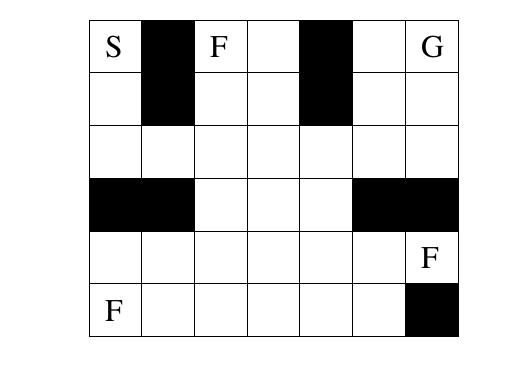
\includegraphics[width=.7\linewidth]{taxi_domain.png}
 \caption{Taxi domain taken from ~\cite{Dearden98bayesianq-learning}, where it appears as the Maze domain.} ~
 \label{fig:taxi_domain}
\end{figure}
\begin{figure}
 \includegraphics[width=\linewidth]{Taxi/learning_curve.pdf}
 \caption{Online and offline scores in the Taxi domain.}
 \label{fig:taxi_learning_curve}
\end{figure}
Figure~\ref{fig:taxi_learning_curve} shows the results of our tests in the Taxi domain. We considered again 100 training episodes, but with 5000 training steps each. We increased the size of the training periods to allow the agent to reach the goal multiple times in the first steps. We found that smaller training episodes might prevent the agent from learning, since it will not reach the goal before the end of the episode.\par
We can see immediately that BQL performs extremely badly in this domain. The agent scores zero because it does not learn to reach the goal. Instead it moves around the grid during the whole duration of the experiments. Q-learning with $\epsilon$-greedy also performs poorly as it learns to pick-up only a single passenger. Surprisingly enough, Q-learning with Boltzmann exploration performs better. The best performance is shown by all 4 versions of PQL, which quickly learn to pick-up all the passengers, even if with different learning speeds. Again, the versions using weighted policy are fairly slower than the rest of the algorithms due to the fact that they explore the actions until the uncertainty about their Q-values is low enough. This might lead to unnecessary exploration as in the first two domains.
\subsection{River Swim Domain }
The next domain we consider is the River Swim domain, taken from ~\cite{Strehl2008AnAO}. The environment is shown in Figure ~\ref{fig:riverswim_domain}. The MDP consists of six states numbered 1 to 6. The two actions available to the agent are to swim left or right represented by the edges in the figure. The agent starts in one of the states near the beginning of the row. Swimming to the right (against the current of the river) will more often than not leave the agent in the same state, but will sometimes transition the agent to the right (and with a much smaller probability to the left). Swimming to the left (with the current) always succeeds in moving the agent to the left, until the leftmost state is reached at which point swimming to the left yields a small reward of five units. The agent receives a much larger reward, of ten thousand units, for swimming upstream and reaching the rightmost state. The $(a,p,r)$ labels next to the edges in Figure~\ref{fig:riverswim_domain} represent the action, probability of success and reward tuple. For example, the label (1,0.7,0) next to the edge from node 0 to node 0 means that when executing action 1 from state 0 there is a 0.7 probability of staying in node 0 and receiving reward 0 and a 0.3 probability of transitioning to state 1 and receiving again reward 0.\par
\begin{figure}
 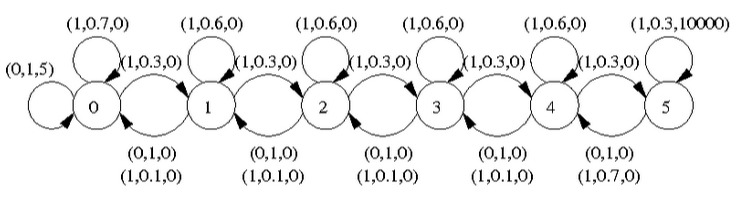
\includegraphics[width=\linewidth]{riverswim_domain.jpeg}
 \caption{River Swim domain taken from ~\cite{Strehl2008AnAO}.} ~
 \label{fig:riverswim_domain}
\end{figure}
\begin{figure}
 \includegraphics[width=\linewidth]{RiverSwim/learning_curve.pdf}
 \caption{Online and offline scores in the River Swim domain.}
 \label{fig:riverswim_learning_curve}
\end{figure}
Figure~\ref{fig:riverswim_learning_curve} shows the results of our tests in the River Swim domain. The length of the training episodes is 1000 timesteps. We train each agent for 100 episodes and show the undiscounted online and offline scores. This domain is the first of our tests where the simple exploration methods completely fail. \par
\begin{figure}
\centering
\begin{subfigure}{\linewidth}
  \centering
  \includegraphics[width=\linewidth]{RiverSwim/particles_weighted-weighted.pdf}
  \label{fig:riverswim_particles_weighted_weighted}
  \caption{}
\end{subfigure}

\bigskip
\centering
\begin{subfigure}{\linewidth}
  \centering
  \includegraphics[width=\linewidth]{RiverSwim/particles_vpi-mean.pdf}
  \caption{}
  \label{fig:riverswim_particles_vpi_mean}
\end{subfigure}
\caption{Evolution of the particles in the first state of the RiverSwim domain during the learning process for the Particle Q-learning algorithm with weighted policy and weighted update (a), and VPI policy and maximum mean update (b). The optimal action is shown on the right, while the suboptimal action is shown on the left on both (a) and (b).}
\label{fig:riverswin_particle_evolution}
\end{figure}
Both Q-learning versions fail to learn the optimal policy. The other algorithms learn fairly quickly. PQL\_V\_M again is the fastest learner. While BQL starts better, is again surpassed in performance by PQL\_W\_W, which learns faster in this domain compared to the previous. This domain has two actions available in every state. Once again we will discuss the evolution of the particles of these two actions in the first state. Figure~\ref{fig:riverswim_particles_vpi_mean} shows how the particles evolve for the same versions of PQL we have investigated in the previous domains. What we can see here, is that the algorithms are robust \wrt the choice of the initialization interval. We can see that, even though the particles are initialized in a large interval, they quickly converge to the true Q-value. This can be seen also in Figure~\ref{fig:riverswim_std_evolution} where the standard deviation of the particles is shown to quickly converge to 0, for both algorithms, for both actions.\par
\begin{figure}
\centering
\begin{subfigure}{\linewidth}
  \centering
  \includegraphics[width=\linewidth]{RiverSwim/std_weighted-weighted.pdf}
  \label{fig:riverswim_std_weighted_weighted}
  \caption{}
\end{subfigure}%

\bigskip
\centering
\begin{subfigure}{\linewidth}
  \centering
  \includegraphics[width=\linewidth]{RiverSwim/std_vpi-mean.pdf}
  \label{fig:riverswim_std_vpi_mean}
  \caption{}
\end{subfigure}
\caption{Standard deviation of the particles as a function of the learning timestep for the Particle Q-learning algorithm with weighted policy and weighted update (a), and VPI policy and maximum mean update (b) in the RiverSwim domain. The optimal action  is shown on the right, while the suboptimal action is shown on the left on both (a) and (b).}
\label{fig:riverswim_std_evolution}
\end{figure}
Finally, we show, in Figure~\ref{fig:riverswim_prob_evolution}, the probability of exploration in the first state as a function of the learning step. Again, this probability converges to 0.
\begin{figure}
  \centering
  \includegraphics[width=\linewidth]{RiverSwim/prob_weighted-weighted.pdf}
  \label{fig:riverswim_prob_weighted_weighted}
\caption{Probability of exploration as a function of the learning timestep for the Particle Q-learning algorithm with weighted policy and weighted update in the RiverSwim domain.}
\label{fig:riverswim_prob_evolution}
\end{figure}
\subsection{Six Arms Domain}
The next environment is again taken from ~\cite{Strehl2008AnAO}. Six Arms, shown in Figure ~\ref{fig:sixarms_domain}, consists of seven states, one of which is the initial state. For how it is build, Six Arms resembles a multi armed bandit problem. The agent must choose from six different actions. Each action pulls a different arm, with a different payoff probability. When the arm pays off, the agent is sent to another state. Within that new state, large rewards can be obtained. The higher the payoff probability for an arm, the smaller the reward received (from the room the agent is sent to by the arm). In this MDP, a decision maker can make use of smaller amounts of experience on the low paying arms and still perform well.\par
\begin{figure}
 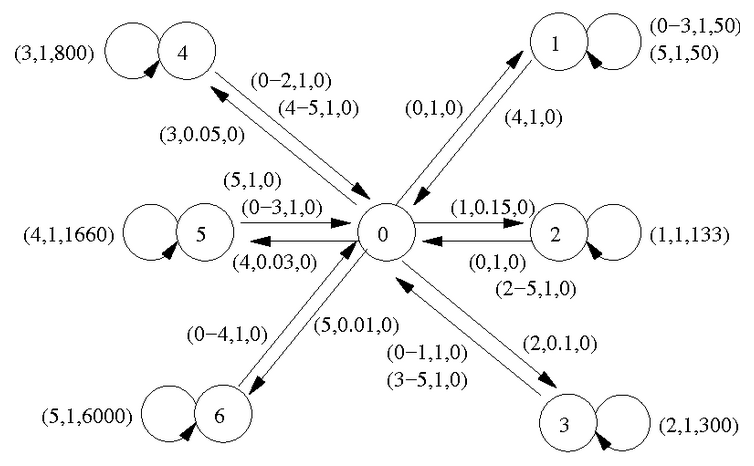
\includegraphics[width=\linewidth]{sixarms_domain.png}
 \caption{Six Arms domain taken from ~\cite{Strehl2008AnAO}.} ~
\label{fig:sixarms_domain}
\end{figure}
Figure~\ref{fig:sixarms_learning_curve} shows the results of our tests in the SixArms domain. Training episodes are the same as in River Swim, Chain and Loop domains. Once again PQL\_V\_M learns faster than the other algorithms. Simple exploration approaches (Boltzmann and $\epsilon$-greedy) fail to learn again. We note the fact that Particle Q-learning with VPI policy and weighted update (PQL\_V\_W) also perform extremely badly. Six Arms is a highly non deterministic domain, and exploration here is really important. VPI policy stops exploration rather quickly and fails to find the optimal actions. We saw this also in the previous domains. The algorithms converged quickly, but the domains were simpler, so VPI policy performed better. PQL\_W\_W on the other hand learns slower than PQL\_V\_M but still better than BQL approaches. BQL with weighted policy seems to have an advantage in the offline setting after the last periods of training, but the behaviour is rather unstable, also due to the uncertainty of the domain itself.
\begin{figure}
 \includegraphics[width=\linewidth]{SixArms/learning_curve.pdf}
 \caption{Online and offline scores in the SixArms domain.}
 \label{fig:sixarms_learning_curve}
\end{figure}
\subsection{Knight Quest}
The last environment we will test our algorithm in is called Knight Quest~\cite{DBLP:conf/icml/FruitPLO18}. This environment takes inspiration from classical arcade games. The goal is to rescue a princess in the shortest time without being killed by the dragon. To achieve this task, the knight needs to collect gold, buy the magic key and reach the princess location. A representation of the game is given in Figure ~\ref{fig:knightquest_domain}.\par
\begin{figure}
 \centering 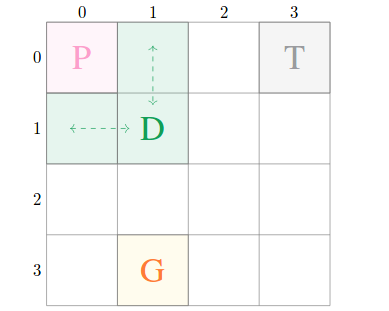
\includegraphics[width=10cm]{knightquest_domain.png}
 \caption{Knight Quest domain taken from ~\cite{DBLP:conf/icml/FruitPLO18}. The green cells are the three locations the dragon can move to.} ~
\label{fig:knightquest_domain}
\end{figure}
The elements of the game are:
\begin{itemize}
\item The knight,
\item the princess,
\item the dragon patrolling the princess,
\item a gold mine,
\item a town.
\end{itemize}
The knight is the only player of the game. He moves in the environment using the four cardinal actions (\ie right, down, left and up) plus an action to keep the current position (stay). Additionally, the knight can collect the gold (collect gold), buy a key (buy key) or buy an armour (buy armour).\par
The town (T) is the place where the knight can buy objects and where it is reset when he rescues the princess or he is killed by the dragon. Saving the princess (P) is the objective, while the gold mine (G) is the place where the knight can collect gold. The dragon (D) is the enemy and it is randomly moving around the princess's location. The dragon can kill the knight when they are at the same position and the knight does not have the armour. We denote as $d \in \{0,1,2\}$ the position of the dragon such that: $d = 0 := (0,1)$, $d= 1 := (1,0)$ and $d= 2 := (1,1)$. The transition probabilities of the dragon are:
\begin{equation*}
p_d(\cdot \vert 0)=[0.4,0,0.6]; \qquad p_d(\cdot \vert 1)=[0,0.4,0.6]; \qquad p_d(\cdot \vert 2)=[0.4,0.2,0.4]. 
\end{equation*}
\par
The state $s_t$ of the game is represented by the following elements:
\begin{itemize}
\item Knight position: coordinates of the grid, $(row,col), \quad row,col \in \{0,1,2,3\};$
\item Gold level: the amount of gold own by the knight, $g \in \{0,1\}$;
\item Dragon position: $d \in \{0,1,2\}$;
\item Object identifier: the object(s) owned by the knight, $o=\{0,1,2,3\}$ where 0 := nothing, 1 := key, 2 := armour and 3 :=key and armour.
\end{itemize}
The movement actions have the trivial effect of changing the knight position. The
action \emph{collect gold} changes the state only when the knight is at the mine. In this case the level of gold is incremented by one, formally $g_{t+1}= \min \{1,g_t + 1\}$. Actions \emph{buy key} and \emph{buy armour} alter the state only when are executed in the town with gold-level equal to 1. All the actions are deterministic when the knight does not own the armour. When the knight has the armour: 
\begin{itemize}
\item The movement actions result in a normal transition with probability 0.5, otherwise the current position is kept;
\item The \emph{collect gold} action fails with probability 0.9, \ie with probability 0.01 the gold level is increment by 1;
\item Actions \emph{buy key} and \emph{buy armour} are not modified.
\end{itemize}
When the knight is equipped with the armour it cannot be killed by the dragon (i.e., knight and dragon can occupy the same cell). At the same time, the armour makes the collection of the goal very challenging (i.e., success probability is 0.01).\par
The basic reward signal is $-1$ at each time step. Nevertheless, the knight receives a reward of $-10$ when he executes \emph{collect gold}, \emph{buy key} or \emph{buy armour} outside the designed location (i.e., mine and town).  The knight obtains a reward of $20$ when he reaches the princess with the key and $-20$ when he is killed by the dragon (i.e., knight and dragon are in the same cell and the knight
does not have the armour). Finally, when the episode ends (i.e., the knight reaches the princess with the key or he is killed), the knight is reset at town location with no gold or object ($g,o= 0$) and the dragon position is randomly drawn, $d \sim U(\{0,1,2\})$.\par
\begin{figure}
 \includegraphics[width=\linewidth]{KnightQuest/learning_curve.pdf}
 \caption{Online and offline scores in the KnightQuest domain.}
 \label{fig:knightQuest_learning_curve}
\end{figure}
Figure~\ref{fig:knightQuest_learning_curve} shows the results of our tests in the KnightQuest domain with the same standard training periods. We can see that in the offline case, simple exploration strategies perform better. Q-learning with Boltzmann and $\epsilon$-greedy exploration quickly reach maximum reward (0 in this domain). Our PQL algorithms learn to achieve maximum rewards also, but slower since they perform exploration. It is interesting that BQL does not reach this maximum reward in the online case, for neither of the policy models. Nonetheless, in the offline evaluations, all algorithms achieve optimal performance rather quickly, with PQL\_W\_W being the slower algorithm. We think these results are due to the fact that this domain is a simple grid-world environment and does not require deep exploration.
\section{Atari Experiments}		 \label{sec:atari_experiments}
In this section we will discuss the results of the ``deep'' version of our algorithm, Particle DQN, and compare its results with Bootstrapped DQN. We chose to compare our results with Bootstrapped DQN because both algorithms perform deep exploration using Q-distributions. Indeed the architecture of the deep network we use to conduct the experiments was taken from ~\cite{DBLP:journals/corr/OsbandBPR16}, which in turn adapts the famous DQN architecture designed by Mnih et al. in ~\cite{mnih2015humanlevel}.\par
We test our algorithms using the Arcade Learning Environment (ALE) described in ~\cite{Bellemare:2013:ALE:2566972.2566979}. Although there is a large number of Atari games we could have tested the algorithms, we present here results obtained in two games, due to the long training time required by the algorithm. It takes three to four days to train the agents in a single Atari game, this by considering training periods only a quarter of the length of the standard of the literature. This is further worsened by the fact that we had to run multiple instances of each algorithm in each environment to show the mean performance over multiple runs (a standard in literature to account for the random initialization of the deep networks).
\subsection{Experimental Setup}
Again we are testing for deep exploration, but in this section we focus in Atari games. Each step of the agent corresponds to four steps of the emulator, where the same action is repeated. The reward values observed by the agents are clipped between -1 and 1 for stability. We evaluate our agents and report performance based upon the raw scores and not the discounted scores. As it is common in literature, we do not show the online performance of the agent during training. We show the scores collected, when exploiting the greedy policies derived from the Q-function after each training period.\par
The \emph{convolutional} part of the network used is identical to the one used in ~\cite{DBLP:journals/corr/OsbandBPR16}. The input to the network is $4\times 84 \times 84$ \emph{tensor} with a rescaled, grayscale version of the last four observations. The first convolutional layer has 32 filters of size 8 with a stride of 4. The second layer has 64 filters of size 4 with stride 2. The last layer has 64 filters of size 3. We split the network beyond the final layer into $N = 20$ distinct heads, each one is fully connected and identical to the network in ~\cite{DBLP:journals/corr/OsbandBPR16}. This consists of a fully connected layer to 512 units followed by another fully connected layer to the Q-Values for each action. The fully connected layers all use \emph{Rectified Linear Units} (ReLU) as a \emph{non-linearity}. We normalize gradients $\frac{1}{N}$ that flow from each head as in ~\cite{DBLP:journals/corr/OsbandBPR16}.
We trained the networks with \emph{RMSProp} optimizer. The discount was set to $\gamma = 0.99$, the number of steps between target updates was set to $\tau= 10000$ steps. We trained the agents for a total of 12.5M steps per game, which corresponds to 50M frames. The agents were evaluated every 1M frames. \par
The \emph{experience replay} contains the 1M most recent transitions. We update the network every 4 steps by randomly sampling a minibatch of 32 transitions from the replay buffer to use the exact same minibatch schedule as Bootstrapped DQN. \par
We show the results of our tests in 3 algorithms: Bootstrapped DQN (Boot\_DQN), Particle DQN with weighted policy and weighted update (P\_DQN\_W\_W), Particle DQN with weighted policy and maximum mean update (P\_DQN\_W\_M). The versions using VPI policy because they did not show good results in preliminary tests. As a result, for time considerations, we did not conduct the full tests on Particle DQN with VPI policy. All algorithms use 20 network heads, \ie we use 20 particles in Particle DQN and $K=20$ in Bootstrapped DQN. We used exactly the same network architecture for all algorithms.
\subsection{Breakout}
In this section we will discuss the experiments conducted on the Breakout Atari 2600 game. A frame from the game is shown in Figure~\ref{fig:breakout_frame}. In this game multiple layers of bricks are positioned in the top of the screen. A ball moves across the screen and bounces at the sides of the screen and at the bricks. When the ball bounces off a brick the brick is removed from the screen and the player gains points. If the ball reaches the bottom of the screen, the player loses a turn. To prevent this from happening the player can move a paddle situated at the bottom of the screen, to bounce the ball back up. The objective of the game is to remove bricks and collect scores as a result. The highest achievable score is 896.\par
We simulated the game through the ALE~\cite{Bellemare:2013:ALE:2566972.2566979}. In the simulator, the game has 4 possible actions. Figure~\ref{fig:breakout_learning_curve} shows the learning curves of the three algorithms considered. We can see that the algorithms have similar performance, with our Particle algorithms scoring slightly higher than Boot\_DQN. An interesting result is that our algorithms seem to be more stable than Boot\_DQN. Being that we implemented the deep networks for both algorithms with the same architecture, if the instability observed in Bootstrapped DQN was a result of the network, we would observe it in all algorithms. This suggests that Particle DQN improved the stability of the agent. 
\begin{figure}
 \centering 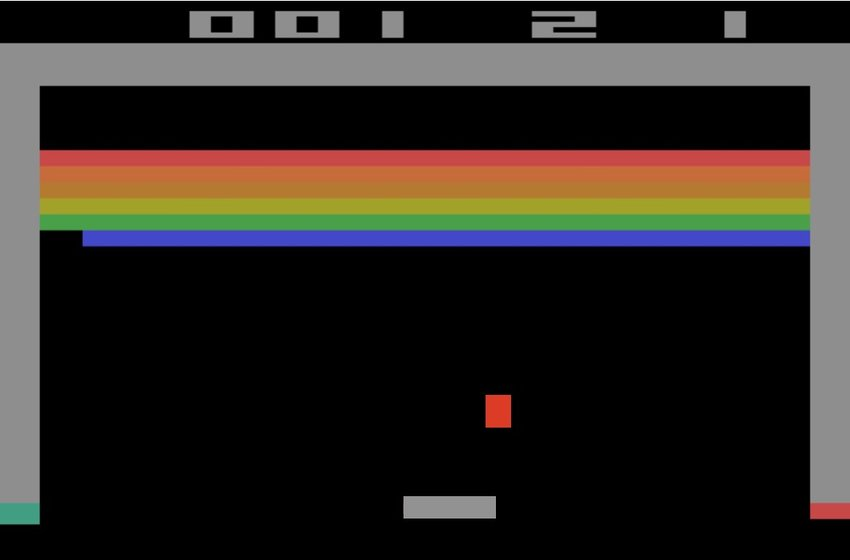
\includegraphics[width=0.7\linewidth]{breakout_frame.jpeg}
 \caption{Frame taken from the Breakout Atari 2600 game.}
 \label{fig:breakout_frame}
\end{figure}
\begin{figure}
 \centering \includegraphics[width=\linewidth]{Breakout/learning_curve.pdf}
 \caption{Evaluation scores in the Breakout Atari 2600 game.}
 \label{fig:breakout_learning_curve}
\end{figure}
\subsection{Montezuma's Revenge}
Breakout is not a game that requires substantial exploration to be played. To test for deep exploration we tested the algorithms in Montezuma's Revenge, a famous Atari 2600 game. In this game, the player controls a character that moves in a 2D world. The character can move between rooms in a underground labyrinth. The objective is to score points by gathering jewels and killing enemies along the way. The agent must find keys to open doors, collect and use equipment such as torches, swords, amulets, etc., and avoid or defeat the challenges in his path.\par
\begin{figure}[H]
 \centering 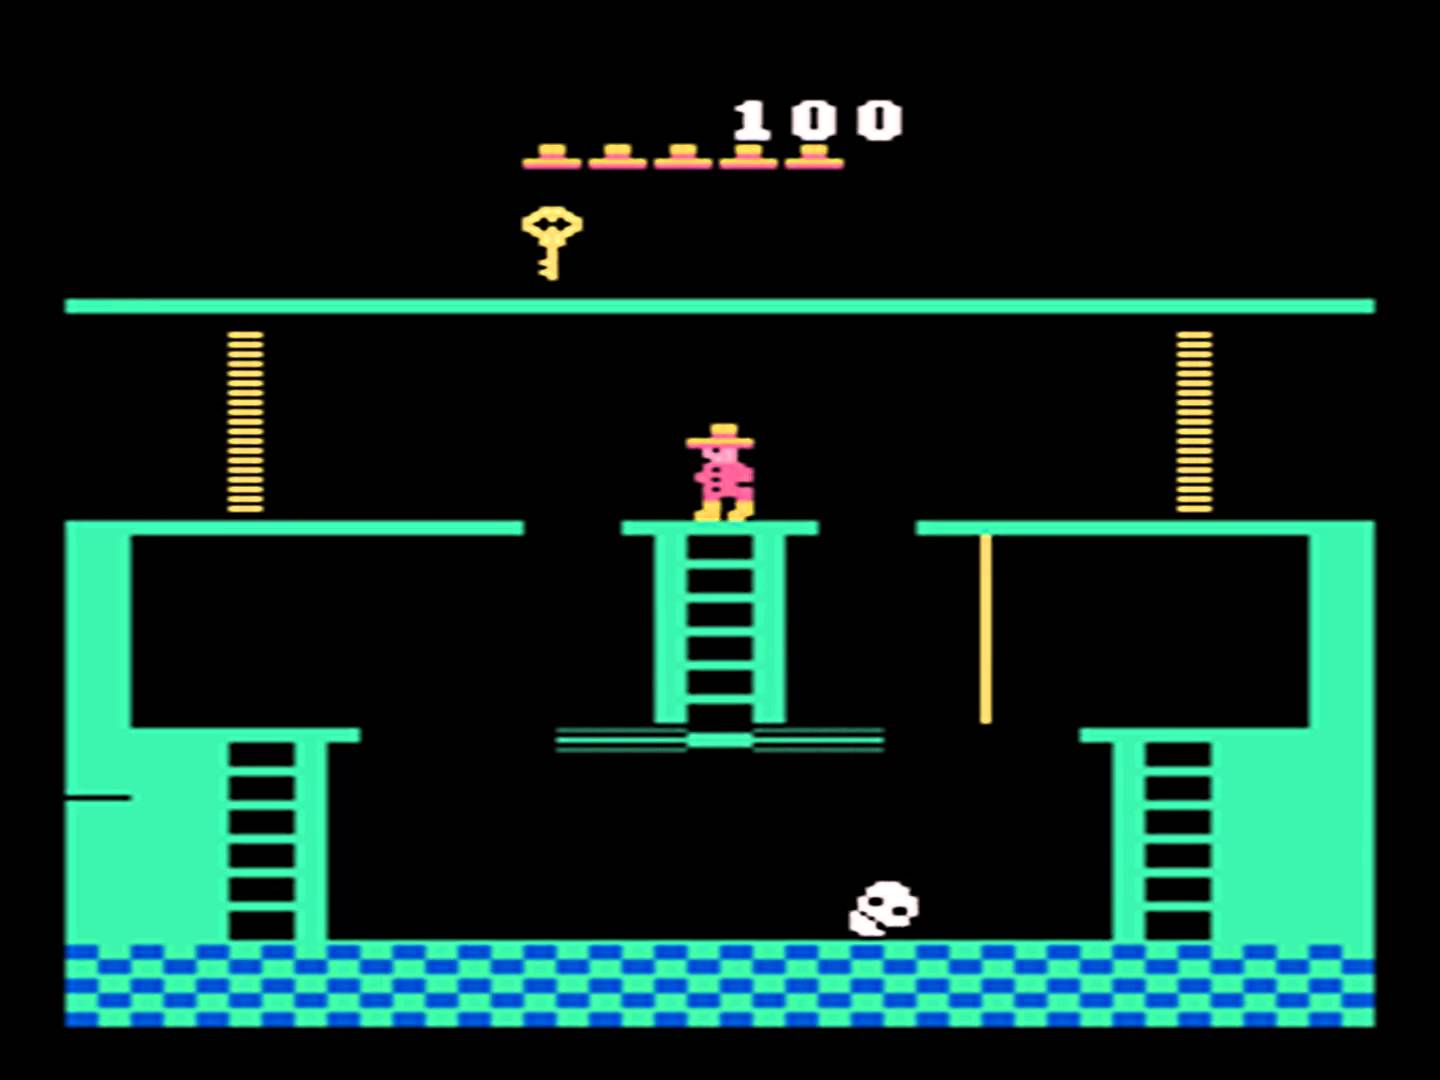
\includegraphics[width=0.7\linewidth]{montezuma_revenge_frame.jpg}
 \caption{Image of the first room of Montezuma's Revenge.}
 \label{fig:montezuma_frame}
\end{figure}
The main characteristic of this game is the scarcity of rewards. As an example, in the first room of the game shown in Figure~\ref{fig:montezuma_frame} the player collects a reward of 100 points when it collects the key, and then another reward of 300 when it opens one of the doors. Reaching the key is extremely difficult, as the agent will die if he falls from a hight or if he touches the enemy (white skull). To move in the following room, the agent needs to follow a very specific route to the key and back to the door. Exploration is extremely important in this domain because the agent requires long sequences of very specific actions to experience any reward, and such sequences are extremely unlikely to occur randomly. As a result, this is considered as one of the most difficult games to beat in the deep RL literature.\par
Figure~\ref{fig:montezuma_learning_curve} shows the results of testing the algorithms in Montezuma's Revenge. Indeed the game lives up to its reputation. Boot\_DQN and P\_DQN\_W\_W fail to score any points in this game. On the other hand, P\_DQN\_W\_M, in all the independent runs, manages to pass to the second room of the game and score 400 points in the process. Unfortunately, the agent does not learn to exploit this in future games. As a result, we see some spikes in the learning curve but no stable growth.
\begin{figure}[H]
 \centering \includegraphics[width=\linewidth]{Montezuma/learning_curve.pdf}
 \caption{Evaluation scores in Montezuma's Revenge.}
 \label{fig:montezuma_learning_curve}
\end{figure}